% Author: Izaak Neutelings (June, 2018)
\documentclass[border=3pt,tikz]{standalone}
\usepackage{ifthen}
\usepackage{siunitx}
\usepackage{tikz}
\usetikzlibrary{hobby} % for ..
\usetikzlibrary{arrows.meta} % to control arrow size
\tikzset{>={Latex[length=4,width=4]}} % for LaTeX arrow head
\usetikzlibrary{calc,intersections,decorations.markings}
\usepackage{siunitx}
\usepackage{xcolor} % for colored text

\colorlet{mylightblue}{blue!20}
\colorlet{myblue}{blue!50!black}
\colorlet{mydarkblue}{blue!30!black}
\colorlet{mylightred}{red!10}
\colorlet{myred}{red!50!black}
\colorlet{mydarkred}{red!60!black}
\colorlet{mydarkgreen}{green!30!black}

%\tikzstyle{midarr}=[decoration={markings,mark=at position 0.5 with {\arrow{stealth}}},postaction={decorate}]
\tikzset{
  midarr/.style={decoration={markings,mark=at position #1 with {\arrow{stealth}}},postaction={decorate}},
  midarr/.default=0.5
}
\def\tick#1#2{\draw[thick] (#1) ++ (#2:0.03*\ymax) --++ (#2-180:0.06*\ymax)}


\begin{document}


% PHASE TRANSITIONS
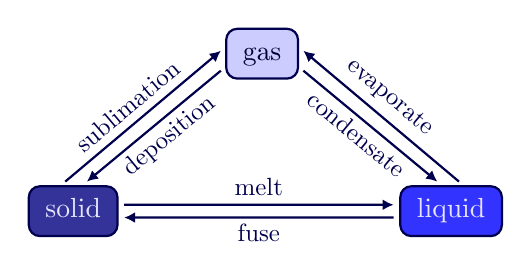
\begin{tikzpicture}[arrow/.style={->,thick,mydarkblue,shorten <=2,shorten >=2},
                    box/.style={thick,rounded corners=4,inner xsep=6,inner ysep=3}]
  \message{Phase transitions^^J}
  
  \node[blue!10!white,draw=mydarkblue,fill=blue!50!gray!80!black,box] (S) at (-2.4,0) {\strut solid};
  \node[blue!10!white,draw=mydarkblue,fill=blue!80!white,box] (L) at (2.4,0) {\strut liquid};
  \node[blue!20!black,draw=mydarkblue,fill=blue!20!white,box] (G) at (0,2) {\strut gas};
  
  \draw[arrow,->] (S.8) -- (L.173) node[above,midway,scale=0.9] {melt};
  \draw[arrow,->] (L.-173) -- (S.-8) node[below=-1pt,midway,scale=0.9] {fuse};
  
  \draw[arrow,->] (S.115) -- (G.-190) node[left=2pt,above,midway,sloped,scale=0.9] {sublimation};
  \draw[arrow,->] (G.-160) -- (S.70) node[left=-2pt,below=-1pt,midway,sloped,scale=0.9] {deposition};
  
  \draw[arrow,->] (L.65) -- (G.10) node[left=2pt,above,midway,sloped,scale=0.9] {evaporate};
  \draw[arrow,->] (G.-20) -- (L.110) node[left=2pt,below=-1pt,midway,sloped,scale=0.9] {condensate};
  
\end{tikzpicture}


% PHASE DIAGRAM
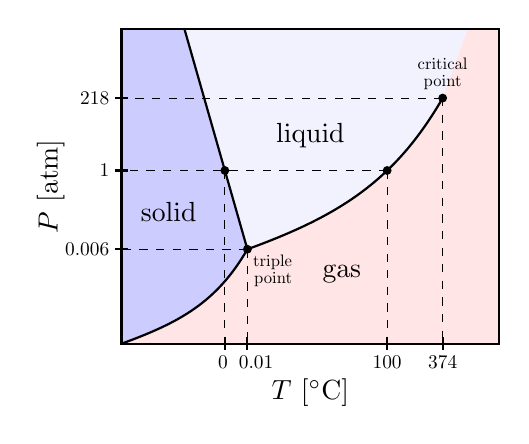
\begin{tikzpicture}[scale=0.4]
  \message{Phase diagrams^^J}
  
  \def\xtick#1#2{\draw[thick] (#1)++(0,.2) --++ (0,-.4) node[below=-.5pt,scale=0.7] {#2};}
  \def\ytick#1#2{\draw[thick] (#1)++(.2,0) --++ (-.4,0) node[left=-.5pt,scale=0.7] {#2};}
  
  % COORDINATES
  \coordinate (O) at (0,0);
  \coordinate (N1) at (2,10);
  \coordinate (N2) at (11,10);
  \coordinate (NE) at (12,10);
  \coordinate (NW) at (0,10);
  \coordinate (SE) at (12,0);
  \coordinate (W) at (0,5);
  \coordinate (S) at (6,0);
  \coordinate (C) at (10.2,7.8); % critical
  \coordinate (T) at (4,3); % triple
  
  % PATHS
  \def\SL{(T) -- (N1)}
  \def\SG{(O) to[out=20,in=-120] (T)}
  \def\LG{(T) to[out=20,in=-120] (C)}
  \def\atm{(0,5.5) -- (12,5.5)}
  \path[name path=SL] \SL;
  \path[name path=LG] \LG;
  \path[name path=atm] \atm;
  
  % REGIONS
  \fill[mylightblue] \SG -- (N1) -- (NW) -- cycle;
  \fill[blue!5] \LG -- (N2) -- (N1) -- cycle;
  \fill[mylightred] \LG -- (N2) -- (NE) -- (SE) -- \SG -- cycle;
  \node at (1.5,4.2) {solid};
  \node at (7,2.2) {gas};
  \node at (6,6.6) {liquid};
  
  %% MIXED
  %\shade[top color=mylightblue,bottom color=mylightred,shading angle=70]
  %  (10.4,7.7) -- (11.2,10) -- (10.8,10) -- (10.0,7.7) -- cycle;
  
  % POINTS
  \fill[black,name intersections={of=SL and atm,by=M}] (M) circle (4pt);
  \fill[black,name intersections={of=LG and atm,by=B}] (B) circle (4pt);
  \fill (T) circle (4pt) node[below right,scale=0.6,align=right] {triple\\[-2pt]point};
  \fill (C) circle (4pt) node[above=1pt,scale=0.6,align=center] {critical\\[-2pt]point};
  
  % LINES
  \draw[thick] \SG;
  \draw[thick] \LG;
  \draw[thick] \SL;
  \draw[dashed] (M) -- ($(M |- 0,0)$) coordinate (Mx);
  \draw[dashed] (T) -- ($(T |- 0,0)$) coordinate (Tx);
  \draw[dashed] (T) -- ($(T -| 0,0)$) coordinate (Ty);
  \draw[dashed] (B) -- ($(B |- 0,0)$) coordinate (Bx);
  \draw[dashed] (B) -- ($(B -| 0,0)$) coordinate (By);
  \draw[dashed] (C) -- ($(C |- 0,0)$) coordinate (Cx);
  \draw[dashed] (C) -- ($(C -| 0,0)$) coordinate (Cy);
  
  % AXES
  \draw[thick] (O) rectangle (NE);
  \node[left=17pt,above,rotate=90] at (W) {$P$ [atm]};
  \node[below=9pt] at (S) {$T$ [\si{\degree C}]};
  \xtick{Mx}{\hspace{-2pt}0}
  \xtick{Tx}{\hspace{9pt}0.01}
  \ytick{Ty}{0.006}
  \xtick{Bx}{100}
  \ytick{By}{1}
  \xtick{Cx}{374}
  \ytick{Cy}{218}
  
\end{tikzpicture}


% PHASE DIAGRAM
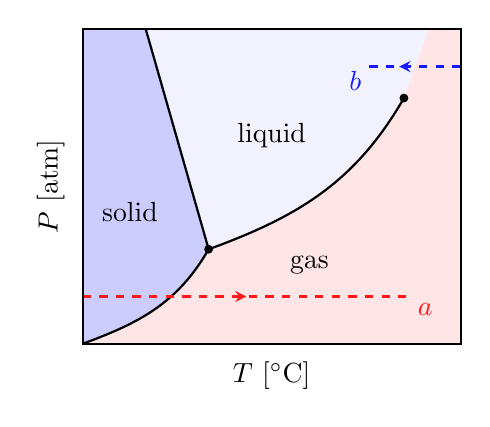
\begin{tikzpicture}[scale=0.4]
  \message{Phase diagrams 2^^J}
  
  \def\xtick#1#2{\draw[thick] (#1)++(0,.2) --++ (0,-.4) node[below=-.5pt,scale=0.7] {#2};}
  \def\ytick#1#2{\draw[thick] (#1)++(.2,0) --++ (-.4,0) node[left=-.5pt,scale=0.7] {#2};}
  
  % COORDINATES
  \coordinate (O) at (0,0);
  \coordinate (N1) at (2,10);
  \coordinate (N2) at (11,10);
  \coordinate (NE) at (12,10);
  \coordinate (NW) at (0,10);
  \coordinate (SE) at (12,0);
  \coordinate (W) at (0,5);
  \coordinate (S) at (6,0);
  \coordinate (C) at (10.2,7.8); % critical
  \coordinate (T) at (4,3); % triple
  
  % PATHS
  \def\SL{(T) -- (N1)}
  \def\SG{(O) to[out=20,in=-120] (T)}
  \def\LG{(T) to[out=20,in=-120] (C)}
  \def\atm{(0,5.5) -- (12,5.5)}
  \path[name path=SL] \SL;
  \path[name path=LG] \LG;
  \path[name path=atm] \atm;
  
  % REGIONS
  \fill[mylightblue] \SG -- (N1) -- (NW) -- cycle;
  \fill[blue!5] \LG -- (N2) -- (N1) -- cycle;
  \fill[mylightred] \LG -- (N2) -- (NE) -- (SE) -- \SG -- cycle;
  \node at (1.5,4.2) {solid};
  \node at (7.2,2.5) {gas};
  \node at (6,6.6) {liquid};
  
  % POINTS
  \fill (T) circle (4pt);
  \fill (C) circle (4pt);
  
  % LINES
  \draw[thick] \SG;
  \draw[thick] \LG;
  \draw[thick] \SL;
  \draw[dashed,red!90,thick,midarr]
    (0,1.5) --++ (10.4,0) node[below right=-1] {$a$};
  \draw[dashed,blue!90,thick,midarr=0.65]
    (12,8.8) --++ (-3,0) node[below left=-2] {$b$};
  
  % AXES
  \draw[thick] (O) rectangle (NE);
  \node[left=3pt,above,rotate=90] at (W) {$P$ [atm]};
  \node[below=3pt] at (S) {$T$ [\si{\degree C}]};
  
\end{tikzpicture}


% PV diagram - isotherms
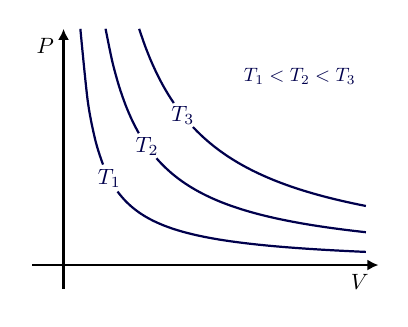
\begin{tikzpicture}
  \message{PV diagram - isotherms^^J}
  \def\tick{0.05*\xmax}
  \def\xmax{4}
  \def\ymax{3}
  \def\N{40}
  \def\isotherm#1#2{{ 1.6*#2/#1 }}
  
  % AXIS
  \draw[->,thick] (0,-0.1*\ymax) -- (0,\ymax)
    node[anchor=north east,inner sep=4,scale=0.8] {$P$};
  \draw[->,thick] (-0.1*\xmax,0) -- (\xmax,0)
    node[anchor=north east,inner sep=4,scale=0.8] {$V$};
  
  % ISOTHERMS
  \path[name path=line] (0,.2*\ymax) -- (.7*\xmax,\ymax);
  \foreach \i/\T in {1/0.4,2/1,3/1.8}{
    \draw[mydarkblue,thick,name path=isotherm\i,
          variable=\x,domain={\isotherm{\ymax}{\T}}:{.96*\xmax},samples=\N,smooth]
      plot (\x,\isotherm{\x}{\T});
    \node[mydarkblue,fill=white,circle,inner sep=0.2,scale=0.8,
          name intersections={of=line and isotherm\i,by=T\i}]
       at (T\i) {$T_\i$};
  }
  
  % LABELS
  \node[mydarkblue,scale=0.7] at (.75*\xmax,.8*\ymax) {$T_1<T_2<T_3$};
    
\end{tikzpicture}


% PV diagram - van der Waals isotherms
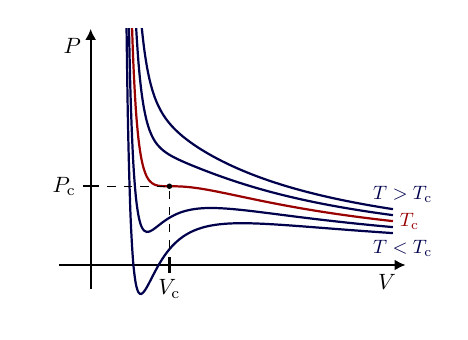
\begin{tikzpicture}
  \message{PV diagram - van der Waals isotherms^^J}
  \def\tick{0.05*\xmax}
  \def\xmax{4}
  \def\ymax{3}
  \def\N{100}
  \def\s{1}
  \def\R{4}
  \def\isotherm#1#2{{ (8*#2)/(3*#1-1) - 3/(#1*#1) }} % reduced equation of state
  \coordinate (C) at (\s,1);
  
  % AXIS
  \draw[->,thick] (0,-0.1*\ymax) -- (0,\ymax)
    node[anchor=north east,inner sep=4,scale=0.8] {$P$};
  \draw[->,thick] (-0.1*\xmax,0) -- (\xmax,0)
    node[anchor=north east,inner sep=4,scale=0.8] {$V$};
  
  % ISOTHERMS
  \begin{scope}
    \clip (-0.2*\xmax,-0.2*\ymax) rectangle (1.11*\xmax,\ymax);
    \foreach \i/\T in {1/0.8,2/0.9,3/1.0,4/1.1,5/1.2}{
      \ifthenelse{\lengthtest{\T pt = 1.0 pt}}{
        \draw[mydarkred,thick,variable=\x,domain=0.36:{.96*\xmax/\s},range=0:1,samples=\N,smooth]
          plot (\s*\x,\isotherm{\x}{\T}) coordinate (EC);
      }{
        \draw[mydarkblue,thick,variable=\x,domain=0.36:{.96*\xmax/\s},range=0:1,samples=\N,smooth]
          plot (\s*\x,\isotherm{\x}{\T}) coordinate (E\i);
      }
    }
  \end{scope}
  
  % LABELS
  \node[mydarkblue,scale=0.7,right=5,below] at (E1) {$T<T_\text{c}$};
  \node[mydarkred,right,scale=0.7] at (EC) {$T_\text{c}$};
  \node[mydarkblue,scale=0.7,right=5,above] at (E5) {$T>T_\text{c}$};
  
  % CRITICAL POINT
  \fill[black] (C) circle (1pt);
  \draw[dashed] (0,1) -- (C) -- (\s,0);
  \draw[thick] (\s,\tick/2) --++ (0,-\tick) node[below=-.5pt,scale=0.8] {$V_\text{c}$};
  \draw[thick] (\tick/2,1) --++ (-\tick,0) node[left=-.5pt,scale=0.8] {$P_\text{c}$};
  
  
\end{tikzpicture}


% PV diagram - Maxwell construction
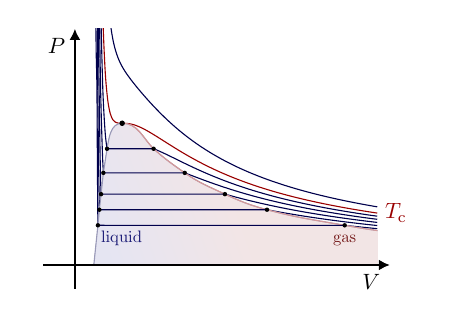
\begin{tikzpicture}
  \message{PV diagram - Maxwell construction^^J}
  \def\xmax{4}
  \def\ymax{3}
  \def\N{110}
  \def\s{0.6}
  \def\A{1.8}
  \def\isotherm#1#2{{ \A*(8*#2)/(3*#1-1) - 3*\A/(#1*#1) }} % reduced equation of state
  \coordinate (C) at (\s,\A);
  
  % LINE
  \foreach \i/\T/\pe in {0/.75/.28,1/.8/.39,2/.85/.5,3/.9/.65,4/.95/.82,5/1.0/1,6/1.1/1}{
    
    \begin{scope}
      \clip (-0.15*\xmax,0) rectangle (1.10*\xmax,\ymax);    
      \ifthenelse{\i = 5}{
        \draw[mydarkred,variable=\x,domain=0.36:{.96*\xmax/\s},range=0:1,samples=\N,smooth,name path=isotherm]
          plot (\s*\x,\isotherm{\x}{\T}) node[mydarkred,right,scale=0.8] {$T_\text{c}$};
      }{
        \draw[mydarkblue,variable=\x,domain=0.36:{.96*\xmax/\s},range=0:1,samples=\N,smooth,name path=isotherm]
          plot (\s*\x,\isotherm{\x}{\T});
      }
      
      \ifthenelse{\i < 5}{ %\lengthtest{\pe pt < 1 pt}
        \path[name path={pe}] (0,\A*\pe) --++ ({.96*\xmax/\s},0);
        \path[name intersections={of=isotherm and pe,name=pe\i}];
      }
      
    \end{scope}
  }
  
  \begin{scope}
    \clip (0,0) rectangle (.96*\xmax,.96*\ymax);
    \fill[top color=myblue!10,bottom color=myred!10,middle color=myred!10,shading angle=110,
          draw=mydarkblue!40,thin,use Hobby shortcut]
      (.06*\xmax,0) -- (pe0-1) -- (pe1-1) -- (pe2-1) -- (pe3-1) --
      (pe4-1) to[out=80,in=180]
      (C) to[out=0,in=135]
      (pe4-3) to[out=-42,in=145]
      (pe3-3) to[out=-35,in=155]
      (pe2-3) to[out=-25,in=165]
      (pe1-3) to[out=-15,in=170]
      (pe0-3) to[out=-10,in=172]
      (.97*\xmax,.144*\ymax) |- (0,0);
    \draw[mydarkred!40,thin,use Hobby shortcut]
      (C) to[out=0,in=135]
      (pe4-3) to[out=-42,in=145]
      (pe3-3) to[out=-35,in=155]
      (pe2-3) to[out=-25,in=165]
      (pe1-3) to[out=-15,in=170]
      (pe0-3) to[out=-10,in=172]
      (.97*\xmax,.144*\ymax) |- (0,0);
  \end{scope}
  \node[blue!40!black!90,below right=-1,scale=0.6] at (pe0-1) {\strut liquid};
  \node[red!40!black!90,below=-1,scale=0.6] at (pe0-3) {\strut gas};
  
  % MAXWELL CONSTRUCTION
  \fill (C) circle (1pt);
  \foreach \i in {0,1,2,3,4}{
    \draw[thin,mydarkblue] (pe\i-1) -- (pe\i-3);
    \fill[black] (pe\i-3) circle (.8pt);
    \fill[black] (pe\i-1) circle (.8pt);
  }
  
  % AXIS
  \draw[->,thick] (0,-0.1*\ymax) -- (0,\ymax)
    node[anchor=north east,inner sep=4,scale=0.8] {$P$};
  \draw[->,thick] (-0.1*\xmax,0) -- (\xmax,0)
    node[anchor=north east,inner sep=4,scale=0.8] {$V$};
  
\end{tikzpicture}


%%% PV diagram - van der Waals isotherms (PGF)
%%\begin{tikzpicture}
%%  \def\N{40}
%%  \def\xmax{4}
%%  \def\ymax{3}
%%  \begin{axis}[every axis plot post/.append style={
%%               mark=none,domain=0.1:\xmax,samples=\N,smooth},
%%               xmin=(-.05*\xmax), xmax=(1.05*\xmax),
%%               ymin=(-.08*\ymax), ymax=(1.08*\ymax),
%%               restrict y to domain=-\ymax:\ymax,
%%               axis lines=middle,
%%               axis line style=thick,
%%               ticks=none,
%%               xlabel={$V$},
%%               ylabel={$P$},
%%               xlabel style={at={(rel axis cs:0.5,0)},below=-2pt,font=\small},
%%               ylabel style={at={(rel axis cs:-0.1,0.5)},rotate=90},
%%               width=9cm, height=7cm,
%%               %clip=false
%%              ]
%%    \addplot plot {8*1/(3*x-1) - 3/x^2};
%%    
%%    \addplot[domain=0:\ymax, samples=90] {max(0,8*2/(3*x-1) - 3/x^2)};
%%    
%%  \end{axis}
%%\end{tikzpicture}


% PHASE TRANSITIONS - ice -> water -> steam
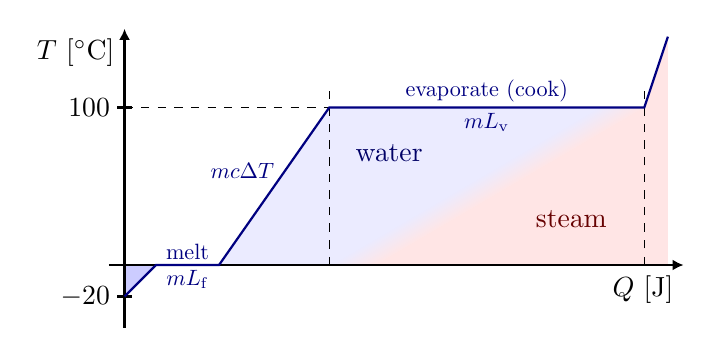
\begin{tikzpicture}
  \message{Phase transition of ice -> water -> steam^^J}
  \def\ymin{-0.8}
  \def\ymax{3}
  \def\xmin{-0.2}
  \def\xmax{7}
  \def\t{0.3}    % water/steam transition zone
  \def\ang{30.4} % angle gradient
  \coordinate (O) at (0,0);
  \coordinate (I) at (0.0,-0.4); % ice
  \coordinate (M) at (0.4,0.0);  % melting
  \coordinate (W) at (1.2,0.0);  % water
  \coordinate (E) at (2.6,2,0);  % evaporate
  \coordinate (S) at (6.6,2.0);  % steam
  \coordinate (F) at (6.9,2.9);  % final
  \coordinate (Ex) at ($(E|-O)$); % x evaporation
  \coordinate (Ey) at ($(E-|O)$); % y evaporation
  \coordinate (Sx) at ($(S|-O)$); % x steam
  \coordinate (Fx) at ($(F|-O)$);
  
  % AREA
  \fill[mylightblue] (O) -- (I) -- (M) -- cycle;
  \fill[blue!8] (W) -- (Ex) -- (S) -- (E) -- cycle;
  \fill[mylightred] (Ex) -- (S) -- (F) -- (Fx) -- cycle;
  \begin{scope} % fade/gradient border
    \clip (Ex) -- (Sx) -- (S) -- (E) -- cycle; % clip gradient rectangle
    \draw[draw=none,transform canvas={rotate=\ang},top color=blue!8,bottom color=mylightred,shading angle=0]
      ({2.6*cos(\ang)},{-2.6*sin(\ang)-\t}) rectangle++(0.65*\xmax,\t); % diagonal border 
  \end{scope}
  \node[blue!40!black,left=4,below right=10] at (E) {water};
  \node[red!40!black,above left=10] at (Sx) {steam};
  
  % AXES
  \draw[->,thick] (0,\ymin) -- (0,\ymax) node[below left=0] {$T$ [\si{\degree C}]};
  \draw[->,thick] (\xmin,0) -- (\xmax+0.1,0) node[below left=0] {$Q$ [J]}; %[\si{J}]
  \draw[dashed] (Ex) -- (E) --++ (0,0.1*\ymax);
  \draw[dashed] (Ey) -- (E);
  \draw[dashed] (Sx) -- (S) --++ (0,0.1*\ymax);
  \tick{I}{0} node[left=-1] {$-20$};
  \tick{Ey}{0} node[left=-1] {$100$};
  
  \draw[dashed] (E) -- (Ex);
  \draw[myblue,thick]
    (I) -- (M) -- (W)
      node[midway,above=-1,scale=0.8] {melt}
      node[midway,below=-1,scale=0.8] {$mL_\mathrm{f}$} --
    (E)
      node[pos=0.6,left=1,scale=0.8] {$mc\Delta T$} --
    (S)
      node[midway,above=-1,scale=0.8] {evaporate (cook)}
      node[midway,below=-1,scale=0.8] {$mL_\mathrm{v}$} --
    (F);
  
\end{tikzpicture}


\end{document}
